\section{グラフの作成方法}
今回のグラフの対象は画像データであり、通常格子状で表現される。そのため、画像の各ピクセルの上下左右のピクセルと連結させたグラフを構築した。

また、ピクセル毎に輝度値が割り振られているため、上下左右でのピクセル間の輝度値の差分$+1$をグラフの辺の重みとした。$1$は輝度値の差が$0$であった場合に連結されてないとみなされないためのバイアス項である。

実装では{\it adjacency\_matrix}関数での{\it to\_abs}関数が辺の重み付けを行っている。


\section{低域通過フィルタの応答}\label{sec:filter}
低域通過フィルタの応答を以下に示す。グラフ周波数領域で、$\lambda$が一定値を超えた際に出力が$0$になるようなステップ関数として実装した。画像では{Original}の波形である。しきい値が3であり、$\lambda < 3$であるあいだは$1$を返し、$\lambda\geq3$では0を返す。

$k=5, 10,\cdots, 25, 50$はチェビシェフ多項式近似による低域通過フィルタであり、$k$は近似式の次数を表す。
\begin{figure}[h]
  \centering
  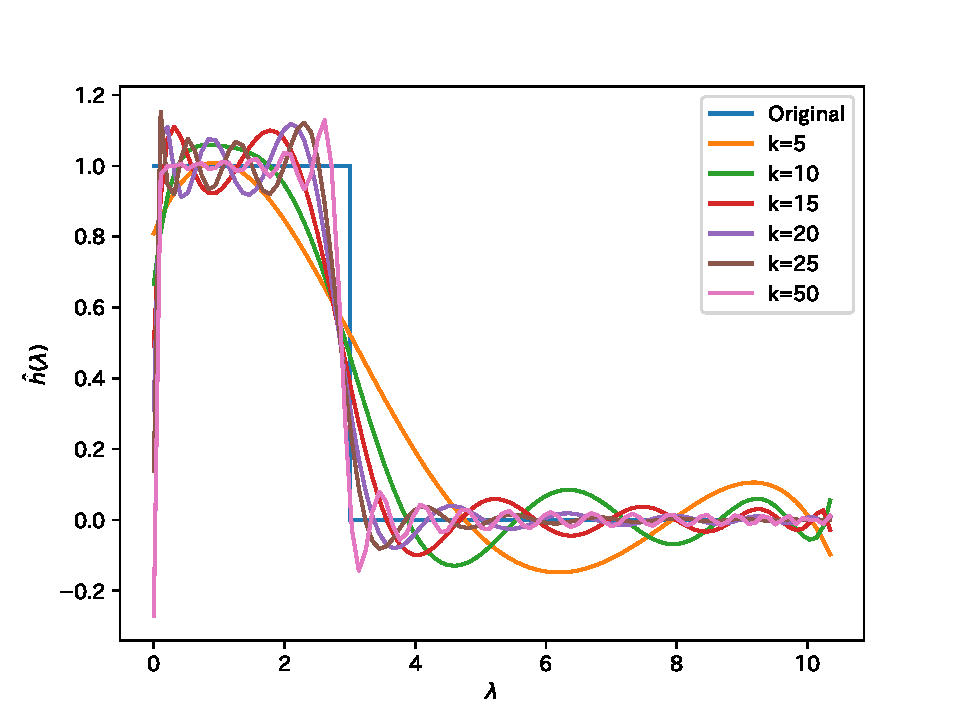
\includegraphics[width=0.95\linewidth]{fig/filter_response.pdf}
  \caption{グラフ周波数領域での低域通過フィルタ}
  \label{fig:filter_res}
\end{figure}

\newpage
\section{入力画像}
入力画像はMNISTデータセットを使用した。

\begin{figure}[h]
  \centering
  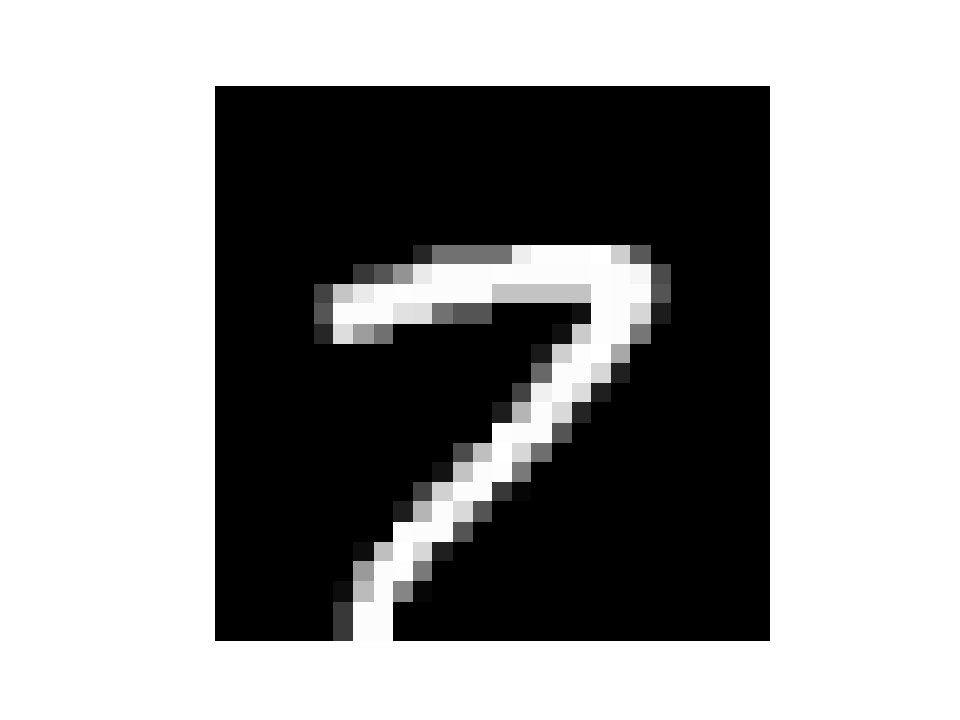
\includegraphics[width=0.3\linewidth]{fig/base_image.pdf}
  \caption{入力画像}
  \label{fig:inputs}
\end{figure}

\section{出力画像}
入力画像に低域通過フィルタを適用した結果を以下に示す。

以下はチェビシェフ多項式近似による低域通過フィルタを適用した際の画像である。次数が増えるにつれ図\ref{fig:filter_res}でも見られるような振動が画像に含まれているのが見て取れる。

\begin{figure}[h]
  \centering
  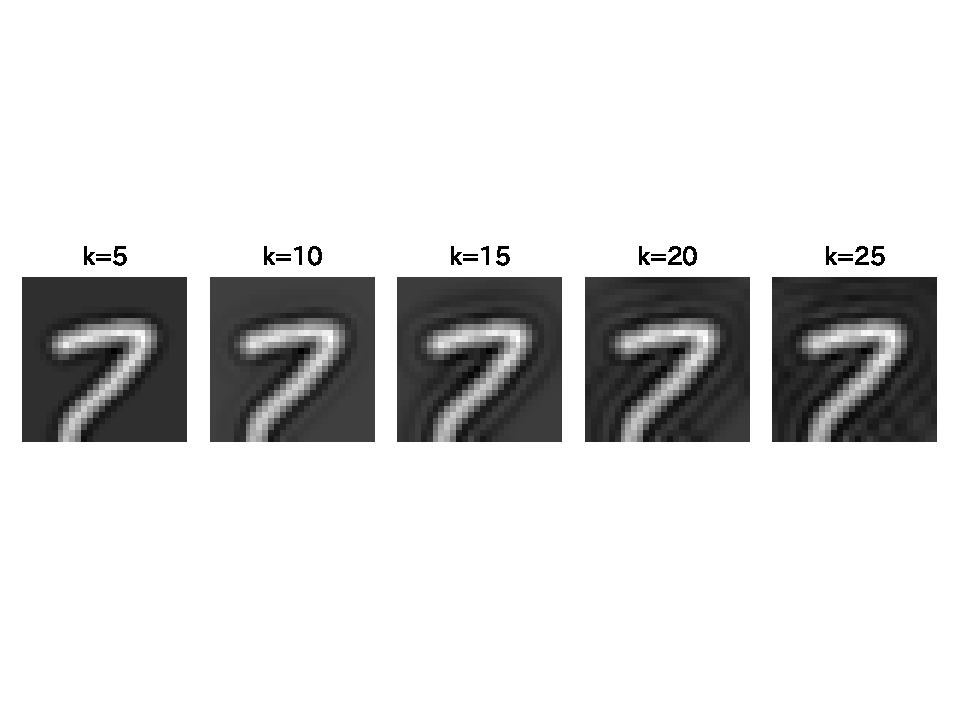
\includegraphics[width=0.7\linewidth]{fig/output_crop.pdf}
  \caption{次数を変化させた出力画像}
  \label{fig:outputs}
\end{figure}


以下は低域通過フィルタのしきい値を変化させた際の画像である。
各画像の上の数値は\ref{sec:filter}低域通過フィルタの応答 で示したしきい値である。

$\lambda$の値が大きくなるにつれぼやけていたエッジが明確になっていく、つまり高周波な信号が含まれていることが確認できる。
\begin{figure}[h]
  \centering
  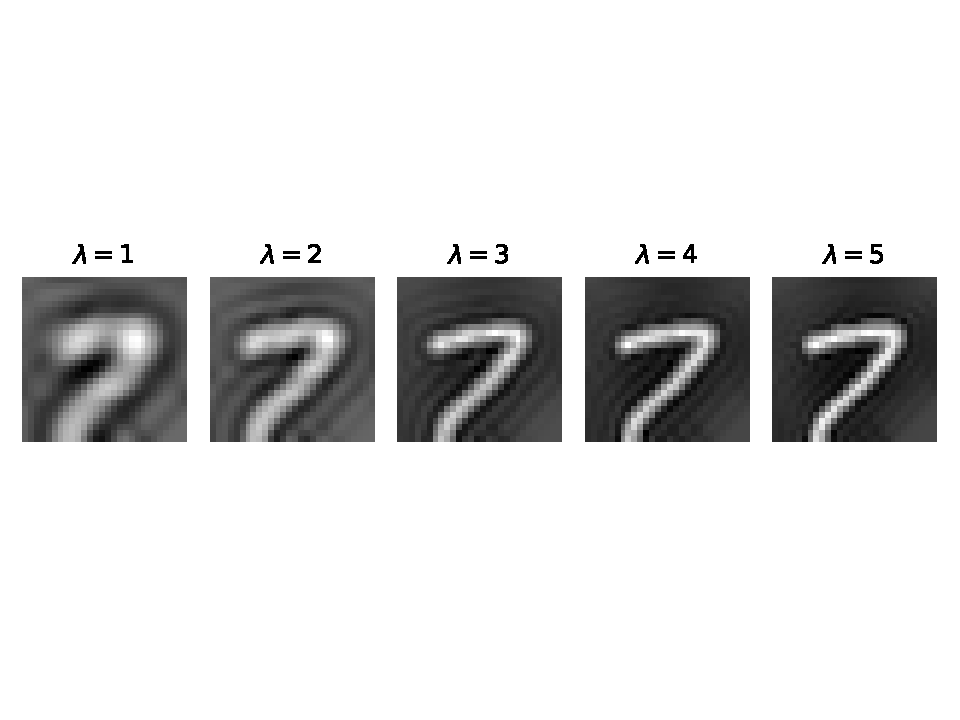
\includegraphics[width=0.7\linewidth]{fig/thershold_crop.pdf}
  \caption{出力画像}
  \label{fig:thresholds}
\end{figure}

\newpage
\section{参考文献}

田中雄一. グラフ信号処理の基礎と応用. コロナ社, 2023.

``PyGSP: Graph Signal Processing in Python''.PyGSP.2017.\url{https://pygsp.readthedocs.io/en/stable/index.html},(参照 2024-07-07)

\section{ソースコード}
実験に使用したプログラムを以下に示す。ソースコード1のload\_mnist.pyではmnistデータセットを取得している。
ソースコード2のmain.pyに含まれる{\it GraphLowPassFilter}がチェビシェフ多項式近似による低域通過フィルタの処理を行っている。

\lstinputlisting[caption={load\_mnist.py}]{src/load_mnist.py}
\newpage
\lstinputlisting[caption={main.py}]{src/myimplementation.py}
